\documentclass[tikz,border=10pt]{standalone}
\usetikzlibrary{angles,quotes,arrows.meta}

\begin{document}
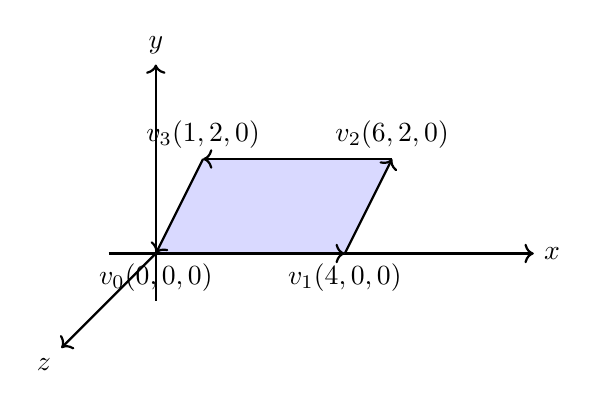
\begin{tikzpicture}[scale=1.2, thick]

% Axes
\draw[->] (-0.5,0) -- (4,0) node[right] {$x$};
\draw[->] (0,-0.5) -- (0,2) node[above] {$y$};
\draw[->] (0,0) -- (-1,-1) node[below left] {$z$};

% Coordinates
\coordinate (v0) at (0,0);
\coordinate (v1) at (2,0);
\coordinate (v2) at (2.5,1);
\coordinate (v3) at (0.5,1);

% Fill the parallelogram
\fill[blue!15] (v0) -- (v1) -- (v2) -- (v3) -- cycle;

% Draw edges with arrowheads
\draw[->] (v0) -- (v1);
\draw[->] (v1) -- (v2);
\draw[->] (v2) -- (v3);
\draw[->] (v3) -- (v0);

% Labels
\node[below]       at (v0) {$v_0(0,0,0)$};
\node[below]       at (v1) {$v_1(4,0,0)$};
\node[above]       at (v2) {$v_2(6,2,0)$};
\node[above]       at (v3) {$v_3(1,2,0)$};

\end{tikzpicture}
\end{document}
